%!TEX root = ./main.tex

\chapter{The quest for a faster kNN search} % (fold)
\label{sec:the_quest_for_a_faster_knn_search}

% TODO: Short intro. The quest is a investigation of ??,  to solve the problem ??. Present the TSI problem.

\section{A short evaluation of OpenCL and CUDA} % (fold)
\label{sub:a_short_evaluation_of_opencl_and_cuda}

As mentioned in Section~\ref{ssub:general_purpose_computing_on_graphics_processing_units}, there are two dominant frameworks for GPGPU programming, CUDA and OpenCL\@. They both have their strengths and weaknesses, and in order to determine which was the most suitable for our work, we performed a small evaluation of both. This evaluation was based on a short benchmark test, where a matrix multiplication application was developed in both frameworks. The development time for both the CUDA and OpenCL matrix multiplier was limited, in order to highlight any differences in ease of use, between the two frameworks.

In addition, a quick analysis of available documentation for both frameworks was made, using common online search engines.

In all our tests CUDA outperformed OpenCL\@. Although our tests were very limited in scope, they support the opinion that currently, CUDA is faster and better documented than OpenCL\@. If the portability offered by OpenCL is not required, we would recommend using CUDA for GPGPU programming.

\subsection{Matrix multiplication benchmark} % (fold)
\label{sub:matrix_multiplication_benchmark}
In order to compare the performance differences between CUDA and OpenCL, a simple matrix multiplication algorithm was implemented in both CUDA and OpenCL\@. These implementations where based on examples provided by NVIDIA and AMD\@. In order to establish a baseline, to which the CUDA and OpenCL results could be compared, additional implementations of the matrix multiplication algorithm was made, as both a naive serial implementation in C and a highly optimized implementation using the Automatically Tuned Linear Algebra Software (ATLAS\cite{atlas}) implementation of BLAS\@. Finally, a highly optimized CUDA implementation was made using the cuBLAS\cite{cublas} library.

The test algorithm multiplies two square matrices of size NxN. This is an interesting problem to use for performance benchmarking for a number of reasons:

\begin{itemize}
    \item Matrix multiplication is often used as a subroutine in more advanced mathematical algorithms.
    \item Matrix multiplication can be parallelized over a large number of computational cores, making it suitable for GPGPU programming.
    \item The mathematics of matrix multiplication is trivial, making it an easy to understand example problem.
\end{itemize}

The four implementations where tested on test environments described in Table~\ref{tbl:test_envoronments}. The results are presented in Figure~\ref{fig:matrix-multiplication-benchmark-results}

\begin{figure}[ht!]
    \centering
    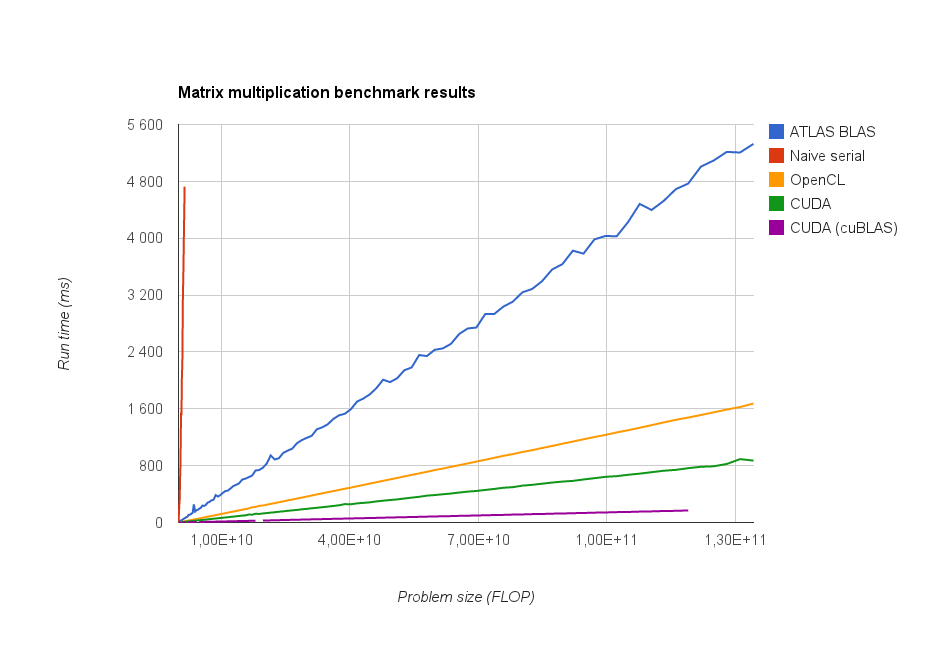
\includegraphics[width=120mm]{../gfx/matrix-multiplication-benchmark-results.png}
    \caption{Matrix multiplication benchmark results}
    \label{fig:matrix-multiplication-benchmark-results}
\end{figure}

We see that the naive serial implementation quickly becomes unusable, due to a rapid increase in run time. The improvement gained by using ATLAS BLAS is very large compared to the naive implementation, although it cannot keep up with the run times achieved by the CUDA and OpenCL implementations.

The difference between CUDA and OpenCL is quite small, compared to the naive and BLAS implementations, but the CUDA implementation is on average about twice as fast as the OpenCL implementation. This is quite a big difference, and this could be related to all tests being run on a NVIDIA graphics card. It might also have been caused by different quality between the NVIDIA and AMD examples.

Looking at the results for the cuBLAS implementation, we can also see the impact of using a highly optimized library for GPGPU programming. The cuBLAS implementation is faster than using the basic CUDA example, indicating that proper use of libraries can be very beneficial.

It is also important to note that this is a very small test. In order to be able to conclude if CUDA is indeed faster than OpenCL, one would have needed to implement a wide selection of algorithms and test them on several different hardware configurations. Although this test is non conclusive regarding this question, the results seem to support several older investigations, concluding that CUDA is faster than OpenCL\@. One notable example being A Comprehensive Performance Comparison of
CUDA and OpenCL\cite{Fang11} by Janbin Fang et al.
% subsection matrix_multiplication_benchmark (end)

\subsection{A quick evaluation of available documentation} % (fold)
\label{sub:a_quick_evaluation_of_available_documentation}

When we where installing CUDA and OpenCL, and implementing our test algorithms, we relied on the online documentation available for the two GPGPU frameworks. Our subjective experience was that finding good documentation for CUDA was a lot easier than for OpenCL\@. In order to investigate this, we made a series of queries for pages related to CUDA and OpenCL on Google, Google scholar and Stackoverflow.com (a popular programming QA site). The results are shown in the following tables (all data from 16. Jan 2014).

\begin{table}[ht]
\centering
    \begin{tabular}{ | l | l |}
    \hline
    \textbf{Query}     & \textbf{No of Stackoverflow.com results}    \\ \hline
    Tagged OpenCL      & 1935                                        \\ \hline
    Tagged CUDA        & 6137                                        \\ \hline
    Open search OpenCL & 5818                                        \\ \hline
    Open search CUDA   & 16174                                       \\ \hline
    \end{tabular}
    \caption{Query results from Stackoverflow}
    \label{fig:stackoverflow-terms-results}
\end{table}

\begin{table}[ht]
\centering
    \begin{tabular}{ | l | l | l |}
    \hline
    \textbf{Query} & \textbf{No of Google results} & \textbf{No of Google Scholar results} \\ \hline
    opencl paralell programming & 322000    & 7480        \\ \hline
    cuda paralell programming   & 558000    & 17100        \\ \hline
    opencl gpgpu                & 558000    & 5230        \\ \hline
    cuda gpgpu                  & 816000    & 13500        \\ \hline
    opencl programming          & 875000    & 8160        \\ \hline
    cuda programming            & 2790000   & 22700        \\ \hline
    \end{tabular}
    \caption{Query results from Google}
    \label{fig:google-terms-results}
\end{table}
% subsection a_quick_evaluation_of_available_documentation (end)
% section a_short_evaluation_of_opencl_and_cuda (end)


\section{Investigation of a brute force approach based on Garcia} % (fold)
\label{sub:investigation_of_a_brute_force_approach_based_on_garcia}

%TODO: General skrytespråk ;-)

%TODO: Revisit this introduction.
As a starting point, for our quest for a fast kNN search, our advisors gave us two papers by Garcia\citep{Garcia2008, Garcia2010}. The topic of these papers are to use a brute force method to solve the kNN problem. Expanding it into a All-kNN solution is then an easy task. These two papers is therefor a perfect start and introduces two new research questions.  

\begin{myrq}
Can high performance be achieved by a parallel brute force kNN algorithm on large point clouds.
\label{rq:brute_force_performance}
\end{myrq}

\begin{myrq}
Can a parallel brute force kNN algorithm be fast enough to solve the All-kNN problem within reasonable time?
\label{rq:brute_force_Q-kNN}
\end{myrq}

\subsection{Garcia's path} % (fold)
\label{sub:garcia_s_effort}

%TODO: Good reference to prev spesification of TSI problem. 
Garcia's effort is based around a more mathematical version of our problem. A mathematician like to generalize a problem and make it a more uniform and accessible to other applications. For example, a mathematician does not make laws for only a 3-d space, but makes a more generalized version in the n-d space. In this case is is by widening the dimensions and not restricting the amounts of neighbors. In short, his problem is to find any number of closest neighbors in a space with any number of dimensions.  

His solution is based around a brute force method. In terms of parallel speedup this would be the best alternative to parallelize the kNN search, because the task can easily be divided into individual subtasks. The brute force, or exhaustive search, algorithm basically consists of three steps:

\begin{enumerate}
       \item Compute all distances between the query point $q$, and all reference points in $S$.
       \item Sort the distances.
       \item Pick the $k$ shortest distances.
\end{enumerate}

If this algorithm is to be used on $n$ query points the time complexity will be \BigO{nmd}. That said, the parallelizable nature of the brute force method makes the speedup, in contrast, potentially high. Even though the speedup is great, and the parallelization is trivial, it does not imply that this is the best approach. Speedup is only a ratio between the parallel and serial speed, so if the algorithm itself is bad the parallel counterpart will also be affected. The brute force approach is steal an interesting candidate for our quest for a fast kNN search.
% subsection garcia_s_effort (end)

\subsection{Continuing on Garcia's path} % (fold)
\label{sub:continuing_on_garcia_s_path} 

Garcia's mathematical path to the kNN problem is good and generic solution, but we need to angle it towards a more specific path. Our problem, in regard to Garcia, is a more engineering-oriented problem. As engineers uses mathematical laws in a more specialized manner, we need to constrain Garcia's problem to fit our specifications. This include a 3-d space with a restricted number of $k$, as described in Section~\ref{a_short_introduction_to_kNN_search_problem}.

First of all, Garcia's implementation only supports problem sizes up to $65535$, as our point clouds tends to be mush bigger, an expansion is therefore necessary. The limitation of $65535$ is exactly the number of theoretical blocks a kernel is allowed to spawn. An expatiation is therefore only a implementation issue, and is solved by a general partitioning algorithm. In short, the algorithm splits a list into a number of partitions. In this case, it is to partition the problem amongst different blocks, as visualized in Algorithm~\ref{alg:general_aspects_dividing}. 
%The whole reimplementation of Garcia's algorithm can be found in Appendix~\ref{sec:brute_force_garcia}.

\begin{algorithm}[ht]
\caption{General work distribution in CUDA}
\label{alg:general_aspects_dividing}
\begin{algorithmic}
\State Let $L$ be any dividable work quantity of size $l$.
    \Function{CUDA-Kernel}{$L$}
    \State $b \gets blockIdx.x$ \Comment{Current block id.}
    \State $d \gets gridDim.x$ \Comment{Numbers of theoretical blocks in current grid.}
    \While{$b<l$}
    \State \Call{do-work}{$L(b)$}
    \State $b \gets b + d$
    \EndWhile
    \EndFunction
\end{algorithmic}
\end{algorithm}

A lot of improvements can be done to Garcia's algorithm, especially if we take advantage of our specialized case. For instance, with the dimension locked to three, the euclidean distance can be calculated in a mush easier fashion.  CUDA consists of lightweight threads, which makes reducing the amount of arithmetic calculations time saving. Garcia, who has to take any number of dimensions into account, uses to vectors and cuBlas to calculate the distance. This makes a lot of extra complexity and data bandwidth, that also can be ignored on our case.

An other, and the most time reducing improvement, has to to with the sorting operation. On a problem instance with a small dimension, the most time consuming operation in Garcia's algorithm is the sorting operation. For instance, a search with $8$ dimensions, the sort occupies $62\%$ of the time \citep[Correct table]{Garcia2008}.
%TODO: Correct citation 

\subsubsection{Bitonic sort} % (fold)
\label{ssub:bitonic_sort}

The best general sorting algorithm today has a time complexity of \BigO{m\ log(m)} \cite{Cormen:2001}, which is a high price to pay for getting the smallest values in a list. One could, as Garcia does, use a sorting algorithm that sorts the list in a linear fashion, where the smallest elements are sorted first. However, this property often gives the soring algorithm a bad time complexity. For instance, Garcia's insertion sort\cite{Cormen:2001} has a time complexity of \BigO{m^2}, and the time complexity of finding the $k$ smallest points would be \BigO{m\ k}. Asymptotically this would give a better timing results in cases where $k$ is smaller then $log(m)$. To get a better understanding of these numbers lets look at an example. If we analyze a case with a $k$ of around $100$. For the insertion sort to get any asymptoticly advantage over the best sorting algorithms, the problem size has to be bigger then $2^{100}$, which is a overwhelming $1.3e30$. We therefore think insertion sort is not the way to go.

Graham Nolan discusses the possibility of improving Garcia's algorithm by using bitonic sort, and he stats that it gave an significant impact\citep{Nolan}. Bitonic sort is a known \BigO{m\ log(m)} algorithm, and is based around a soring network. The network is a series of interleaving bitonic sequences. A sequence is bitonic if it monotonically increases an then monotonically decreases\cite{Cormen:2001}. An iterative version of the bitonic sort is described in Algorithm~\ref{alg:bitonic_sort}.

\begin{algorithm}[ht]
\caption{Iterative Bitonic sort}
\label{alg:bitonic_sort}
\begin{algorithmic}
    \Require{A list $L$ with length $m$.}
    \Ensure{A sorted list, $L$}
    \State $P \gets \{2^i|i \in \mathcal{N} \}$
    \Function{Bitonic-Sort}{$L$}
        \ForAll{$\{p \in P\ |\ p \le m \}$}
            \ForAll{ $\{k \in P\ |\ p \ge k > 0\}$}
                \ForAll{$0 \le i < m)$}
                \State $pos \gets k \veebar p$ \Comment{$\veebar$ is the bitwise $xor$ operator}
                \If{$pos < i$}
                    \If{$\lnot(i \& p)$} \Comment{$\&$ is the bitwise $and$ operator}
                        \State \Call{compare}{$L(i),L(pos)$}
                    \EndIf
                    \If{$(i \& p)$}
                        \State \Call{compare}{$L(pos),L(i)$}
                    \EndIf
                \EndIf
                \EndFor
            \EndFor
        \EndFor
    \EndFunction
    \Statex
    \Function{Compare}{$a,b$}
    \If{$a>b$}
    \State \Call{swap}{$a,b$}
    \EndIf
    \EndFunction
\end{algorithmic}
\end{algorithm}
% subsubsection bitonic_sort (end)

\subsubsection{Min-reduce} % (fold)
\label{ssub:min_reduce}

Sorting the distances, with a \BigO{m\ log(m)} operations, still looks like a high price to pay to get the smallest values. Especially if $k$ is reasonably small. Why do we need to sort the list in the first place? Sorting is a very naive way to go. The problem it solves is also extremely general compared to our specific goal, which is to get the smallest $k$ values. An algorithm that is more suitable, and also highly parallelizable, is a reduce operation. Cormen\cite{Cormen:2001} defines $\otimes$-reduction of an array $d$ of size $m$, where $\otimes$ is any associative operator, to be the value $y$, given by the following formula:

     $$ y = d[1] \otimes d[2] \dots \otimes d[m].$$

In serial this is a typical linear algorithm with time complexity \BigO{m}, as shown in Algorithm~\ref{alg:serial_reduce}. 

\begin{algorithm}[ht]
\caption{Serial $\otimes$-reduction}
\label{alg:serial_reduce}
\begin{algorithmic}
    \State Let $\otimes$ be any associative operator.
    \Function{Reduce}{$d, \otimes$}
        \State $y \gets d[0]$
        \For{$i \gets 1,\, m$}
            \State $y \gets y \otimes d[i]$
        \EndFor
    \EndFunction
\end{algorithmic}
\end{algorithm}

Since the operator $\otimes$ is associative, there is no difference in which way the values are calculated or if it's done on parallel. A tree based approach, like Figure~\ref{fig:paralell_reduce_operation}, could be used. It is a good parallelization strategy, where every possible independent subtask is parallelized. Here each tree level do the associative operations in parallel, the results are combined as the tree level progresses downwards, until only one element remains. The parallel equivalent to Algorithm~\ref{alg:serial_reduce} is therefore done in \BigO{log(n)} time. 

% TODO: finne en tittle
\begin{figure}[ht!]
\centering
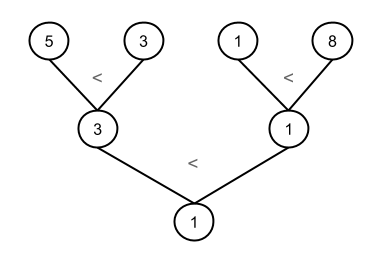
\includegraphics[width=50mm]{../gfx/min_reduce.png}

\caption{A visualization of the parallel min-reduce operation.}
\label{fig:paralell_reduce_operation}
\end{figure}

To solve our problem the associative operation has to be the minimum operator. A min-reduce algorithm is easy to implement in CUDA, but it is hard to get fast. Implementing the min-reduce algorithm can easily be done in CUDA, but in order to get the best performance some optimization techniques, like loop unrolling, sequential addressing and warp unrolling, described in Section~\ref{sec:cuda_optimizations} should be applied.   
% subsubsection min_reduce (end)

\subsubsection{Results} % (fold)
\label{ssub:comparison}

%TODO: More bragging, less Garcia.
Now that we have three different implementations of the kNN brute force method, lets take look at how they compare. Figure~\ref{fig:brute_force} shows the timing results with $k$ equals $10$. Garcia's algorithm lose much time, because of the more general problem it solves and the use of insertion sort. The generality also impacts the number of supported reference points, as the shorted graph implies. Graham Nolan's idea to improve the sorting algorithm gave a huge impact. It is almost five times faster then Garcia's implementation, shown in Table~\ref{tab:tabulated_results_from_brute_force}. Bitonic sort has a soring network that is suited for lengths that is a power of two, which give some pits in the graph. Partitioning of the list amongst the CUDA blocks, also moved the pits a bit around.  

\begin{figure}[ht!]
\centering
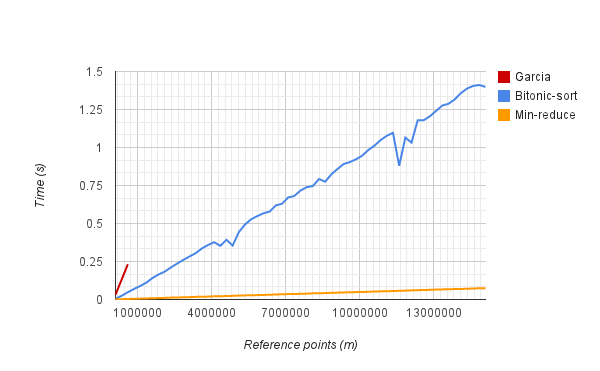
\includegraphics[width=100mm]{../gfx/brute_force.png}

\caption{Three different kNN brute force implementations. The timing results is based on a $k$ equal to $10$.}
\label{fig:brute_force}
\end{figure}

\begin{table}[ht]
\centering
    \begin{tabular}{ | l | l |l |l|}
    \hline
    \textbf{Reference points (m)} &\textbf{Garcia} & \textbf{Bitonic sort} & \textbf{Min-reduce}\\ \hline
    \textbf{\numprint{6.0e5}} & $231.8ms$ & $48.1ms$& $3.3ms$\\ \hline
    \textbf{\numprint{1.1e7}} & -& $1077.2ms$ & $54.2 ms$ \\ \hline
    \end{tabular}
    \caption{Some tabulated results from Figure~\ref{fig:brute_force}.}
    \label{tab:tabulated_results_from_brute_force}
\end{table}

The big winner in this contest is the min-reduce version. It is $70$ times faster then Garcia and almost $15$ times faster then the bitonic version. Although min-reduce is the big winner at a low k, lets not imply that it always is going to be the best alternative before some analysis are made.

First of all, lets see whats happening asymptoticly when $k$ is increasing.  Performing $k$ min-reduce operations takes \BigO{klog(m)} time, because one min-reduce has a time complexity of \BigO{log(m)}. If we increase $k$ towards $m$, the result would be a sorted list, and the time complexity will go towards \BigO{mlog(m)}. This is the same time complexity as our bitonic sort. The asymptotic growth of the min-reduce variant will not be any different then the bitonic sort variant, even though $k$ equals $m$. 

A sorting operation with min-reduce naturally have a bigger constant time penalty than the bitonic version. However, if $k$ is reasonably small, the min-reduce method is highly superior.   
% subsubsection comparison (end)
 % subsection garcia_s_effort (end) 


% section investigation_of_a_brute_force_approach_based_on_garcia (end)

\section{Application of k-d trees to the kNN problem} % (fold)
\label{sub:application_of_kd_trees_to_the_knn_problem}

A common strategy when wanting to improve the performance of repeated queries in a large dataset, is to organize the dataset into some data structure suited for fast querying. This strategy trades the additional time required building an data structure, for increased performance on each query. In Section~\ref{sub:investigation_of_a_brute_force_approach_based_on_garcia} we developed an optimized parallel brute force algorithm for performing kNN queries on a large point cloud. In this section we will investigate the possibility of improving on the brute force algorithm by using the k-d tree data structure.

\begin{myrq}
\label{rq:serial-kd-tree}
    It is possible to use a k-d tree to increase the performance of kNN queries, compared to a parallel brute force solution?
\end{myrq}

\begin{myrq}
\label{rq:serial-kd-tree-all-knn}
    It is possible to use a k-d tree to increase the performance of All-kNN queries, compared to a parallel brute force solution?
\end{myrq}

A brief argument for why k-d trees is well suited for kNN query operations is given, then we will present the k-d tree data structure, and show how it can be used for operating on three-dimensional point cloud data. Finally a set of tests are performed on implementations of the k-d tree based algorithms, in order to determine the possible benefits of a parallel k-d tree based algorithm.

\subsection{Why k-d trees?} % (fold)
\label{sub:why_k_d_trees_}
A large part of this thesis is devoted to applying k-d trees to the kNN problem. The reader might ask themselves why this is so. Other possible data structures exist which is optimized for querying in geometrical data. Why choose to investigate k-d trees in particular?

Part of the explanation has to do with the scope and time resources available for the work in this thesis. Performing a full analysis and parallelization of every possible data structure, and their associated query algorithms, would just not be feasible within our time frame. That said, k-d trees is a very attractive data structure for our use case.

\begin{itemize}
    \item k-d trees are easy to understand and implement, leaving more time to throughly investigate parallelization of the algorithms.
    \item k-d trees are a very minimal data structure, and balanced k-d trees are complete binary trees. This makes reducing the amount of additional memory required in addition to the 3-d points a relative simple task. This is important considering the memory bounds on GPUs, and the time penalty associated with moving data from system memory to GPU memory.
    \item k-d trees are well adapted to performing associative queries, where the query is for a point that is not equal to, but close to the query point.
    \item Studies on parallel kNN queries based on k-d trees has been documented in literature with encouraging results\cite{Owens:2007:ASO,Zhou:2008:RKC:1409060.1409079, Brown2010}.
\end{itemize}
% subsection why_k_d_trees_ (end)

\subsection{Building k-d trees for point cloud data} % (fold)
\label{ssub:building_k_d_trees_for_point_cloud_data}

A k-d tree can be thought of as a binary search tree in k dimensions. A binary search tree is constructed such that, for a given node, one child-subtree is consisting of elements smaller than the current node, and the other child-subtree is consisting of elements larger than the current node. The same strategy is applied when constructing a k-d tree, but at each level we are sorting the child-subtree elements according to one selected dimension, called the discriminant for this level. This discriminant is cycled through the different dimensions, as we move down each level in the tree. A formal description of k-d trees is given by Jon Louis Bentley in the paper Multidimensional Binary Search Trees Used for Associative Searching\cite{Bentley:1975:MBS:361002.361007}.

Let us have a look at an example using data for two dimensions. Figure~\ref{fig:kd_tree_2d_plane} shows us a set of points on a two dimensional plane. The lines through each point indicate the split plane formed by the discriminant associated with the different points.

\begin{figure}[ht!]
    \centering
    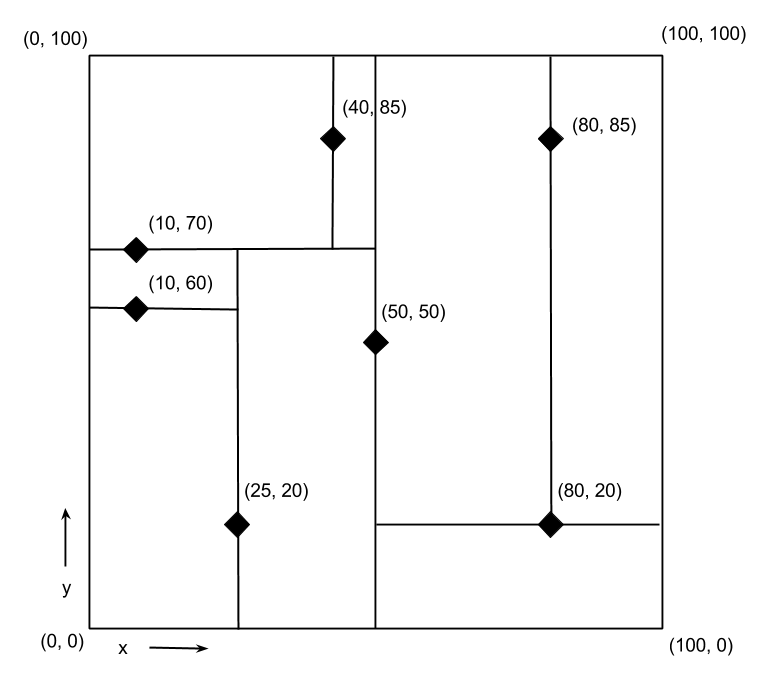
\includegraphics[width=85mm]{../gfx/kd_tree_illustration_graph.png}
    \caption{A set of points on a plane, with a possible k-d tree indicated.}
    \label{fig:kd_tree_2d_plane}
\end{figure}

The corresponding k-d tree is shown in Figure~\ref{fig:kd_tree_2d}. Note that lower values in each level are placed in the left branches, and higher values are placed in the right branches.

\begin{figure}[ht!]
    \centering
    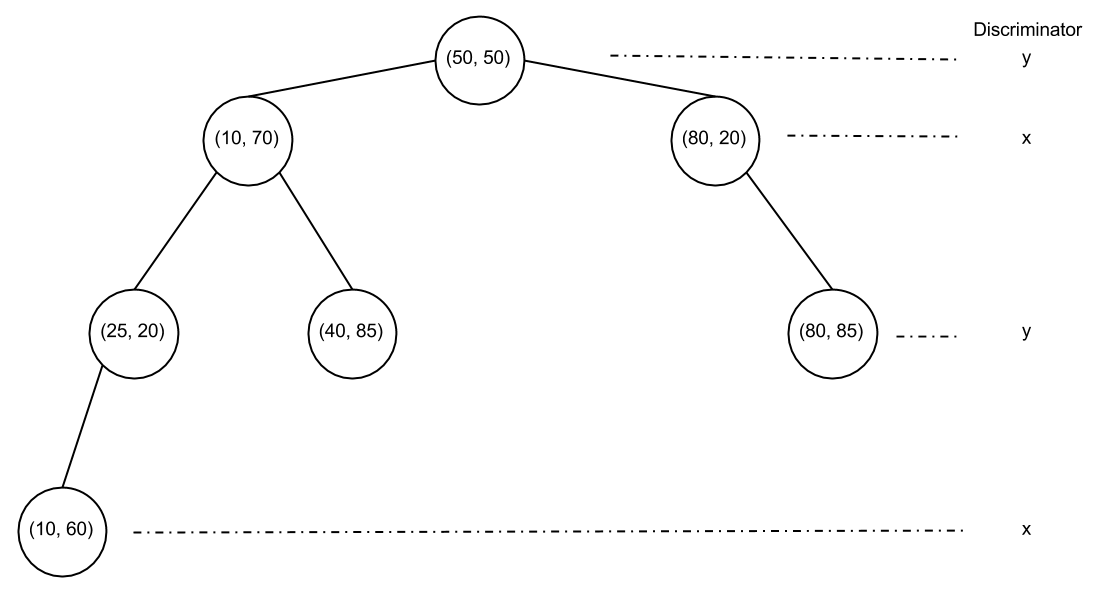
\includegraphics[width=120mm]{../gfx/kd_tree_illustration_tree.png}
    \caption{Tree representation of the points in Figure~\ref{fig:kd_tree_2d_plane}.}
    \label{fig:kd_tree_2d}
\end{figure}

By extending this example with three fixed dimensions for the spatial dimensions, x, y, and z, we get a k-d tree suitable for storing point cloud data.

It it possible to construct several algorithms for building k-d trees from a set of points, and one simple approach is using a recursive function. Algorithm \ref{alg:seriel_tree_build} shows pseudocode for such a simple tree building algorithm. In the pseudocode, we have chosen to represent the different dimensions as a natural number. This means that x is represented by 0, y is represented by 1, z is represented by 2 and so on. Given a set of point, $P$, in $k$ space, and a initial split dimension $i$, it constructs a balanced k-d tree.

\begin{algorithm}
\caption{Recursive k-d tree build}
\label{alg:seriel_tree_build}
\begin{algorithmic}
    \Function{Build-KD-Tree}{$P$, $i$}
        \If{$P.length = 0$} \Comment{We have reached the end of a branch}
            \State \textbf{return} NIL
        \Else
            \State $m \gets \text{Median}(P)$

            \State \text{Let $L$ be all elements of $P < m$ in dimension $i$}
            \State \text{Let $H$ be all elements of $P > m$ in dimension $i$}

            \State $i' \gets (i + 1) \bmod k$ \Comment{k = 3 for a three dimensional k-d tree}

            \State $m.left \gets \text{Build-KD-Tree}(L, i')$
            \State $m.right \gets \text{Build-KD-Tree}(H, i')$
        \EndIf
        \State \textbf{return} $m$
    \EndFunction
\end{algorithmic}
\end{algorithm}

Algorithm~\ref{alg:seriel_tree_build} starts by checking if there is any more points left in $P$. If not, it returns NIL as an end of branch marker. If there still is points left, the algorithm selects the median point, $m$, as the root node. Then it sorts all remaining points into a collection of points lower than the median, $L$, and higher than the median, $H$. The dimension, $i$, is incremented, and the Build-KD-Tree function is called recursively on both collections of points. Finally the root node is returned, so it can be assigned as the child of it's parent node, or be used as a global root node.

It is worth to note that the performance of this k-d tree build algorithm is sensitive to the choice of a median finding algorithm, since we will be querying for the median \BigO{m} times. Choosing to just sorting the collection $P$, and selecting the median from the middle of the sorted collection, will not give optimal results. Fortunately, several \BigO{m} median selecting algorithms exist\cite{Cormen:2001} (Get chapter citation), quickselect, being the choice for our initial implementations. Given a fixed number of dimensions, this gives a algorithm with a time complexity of \BigO{m\ log(m)}\cite{Friedman:1977}.

A final note about Algorithm~\ref{alg:seriel_tree_build}, is that it does not handles points with duplicate values in one dimension. If the algorithm where to be feed with a point collection where all points had the same value for x, it would not be able to handle it, since such a point does not explicitly belong in $L$ or $H$. Several modifications can be made to handle this case. We can choose to place all conflicting median points, except one, in either $L$ or $H$. The problem with this solution, is that we are not guaranteed to get a balance tree. If we where to have a set of points, where all points where tha same, we would get a tree at all, but just one long branch of length n. Another strategy is to try to place the conflicting medians, equally in $L$ and $H$. This way the median we select will be the midmost element in the point collection, retaining the balance in the finished k-d tree. Given that we consider that duplicate median points can be located in both subtrees of a node, this will not affect search operations on the tree, as we will see later.
% subsection building_k_d_trees_for_point_cloud_data (end)

\subsection{Querying the k-d tree}  % (fold)
\label{sub:querying_the_k_d_tree} 

With a k-d tree we can perform efficient searches for the closest point to a given point in \BigO{log(m)} average time\cite{Friedman:1977}. By maintaining a collection of the k closest points during execution of the query, we can even perform kNN searches. An example of a kNN search algorithm is shown in Algorithm~\ref{alg:recursive_knn_kd_tree_search}.

%TODO: Something about how searching works in the general sense?

The procedure will take the root of a k-d tree, $r$ and a query point, for which we want to find the k closest points. In addition, it requires a initial dimension, $i$, which should be the same as the initial dimension used when building the tree. It uses this data to manipulate a collection of the k closest points to $q$. This collection is called the k-heap, $K$.

The k-heap is a data structure with some special properties. You can query it for the maximum distance value of the k points stored in it, and it will only store a predetermined number of points. If you try to insert more points than the predetermined number of points, it will discard the highest values, and only keep the k lowest values. This data structure can be easily implemented as a modified max-heap\citep[Chapter 6]{Cormen:2001}. When the size of the heap is lower than k, it is used in the usual manner, but when the heap is of size k, a slight modification to the insertion operation is made. Instead of adding the new element to the heap, the new element is swapped with the maximum value of the heap, if it is lower than the current maximum value in the k-heap. Then the heap is re-balanced using the standard max-heap balance algorithm. In our code, we assume the k-heap to be filled at the start with k points of either a random sample of points from the k-d tree, or with positive infinity. This way we do not need to check if the heap is filled during the recursive execution of the procedure.

\begin{algorithm}
\caption{Recursive kNN k-d tree search}
\label{alg:recursive_knn_kd_tree_search}
\begin{algorithmic}
    \Procedure{kNN-KD-Tree}{$K, r, q, i$}
        \If{$r =$ NIL} \Comment{We have reached the end of a branch}
            \State \textbf{return}
        \EndIf

        \State $d \gets \text{Distance}(r, q)$
        \State $dx \gets r.x[i] - q.x[i]$

        \If{$d < K.max$} \Comment{Is $r$ closer to $q$ than the current k best points?}
            \State $r.distance \gets d$
            \State \text{Insert}($K, r$)
        \EndIf

        \State $i' \gets (i + 1) \bmod k$ \Comment{k = 3 for a three dimensional k-d tree}

        \If{$dx > 0$}  \Comment{Select $t$ and $o$ so we traverse towards closest point first}
            \State $t \gets r.left$, $o \gets r.right$
        \Else
            \State $t \gets r.right$, $o \gets r.left$
        \EndIf

        \State \text{kNN-KD-Tree} ($K, t, q, i'$)

        \If{$dx^2 < K.max$} \Comment{Can there be closer points in the other subtree?}
            \State \text{kNN-KD-Tree}($K, o, q, i'$)
        \EndIf
    \EndProcedure
\end{algorithmic}
\end{algorithm}

Algorithm \ref{alg:recursive_knn_kd_tree_search} starts by checking if we have reached the end of a branch. If not, it calculates the Euclidean distance between the query point, $q$, and the current root point, $r$. Calculating this distance is a costly step, since it usually involves calculating a square root. This can be circumvented when implementing, by relying on using the square of the Euclidean distance as the distance metric, instead of the actual distance. This will not make a difference for the algorithm. The distance, $dx$, between the current root and the query point in dimension $i$ is also calculated.

The algorithm then checks if the current root point is closer to the query point than one of the points in the k-heap. If this is the case, it inserts the current root into the k-heap. The next dimension, $i'$, is calculated, and then the algorithm determines if it should traverse to the right or left child node first. For efficient querying, we want to traverse down the branch that would contain the query point. In other words, if the query point is lower than the current root point in the current dimension, we want to traverse to the left child, and vice versa. The child node that we want to traverse first, is often called the target, and it's corresponding subtree is often called the target subtree. In the algorithm the symbol $t$ is used to represent target. The child and child-subtree that is not chosen for immediate traversal is called other and other-subtree. In the algorithm the symbol $o$ is used to represent other. The ability to prune away the other subtree, given our current best estimates stored in the k-heap and the distance $dx$, is what makes the k-d tree efficient for kNN searches.

After recursively investigating the target subtree, we ask if our estimates in the k-heap is better than the distance $dx$, remembering that the distances stored in the k-heap is squared. If this is the case, we know that there cannot be a closer point in the other subtree, and we can prune it from our search. If not, we have to check the other subtree as well. When the procedure terminated, the k closest points to the query point is stored in the k-heap.
% subsection querying_the_k_d_tree (end)

\subsection{Testing a serial k-d tree based kNN solver} % (fold)
\label{sub:testing_a_serial_k_d_tree_based_knn_solver}

%TODO: Add in appendix and reference.
In order to gain some real world insight into the performance characteristics of k-d tree building and querying, a serial implementation of the build and query algorithm was made. This implementation is available in Appendix X. These two implementations where then subjected to several tests, using test setup Y. All tests were performed on a set of randomly generated points 3-d points, with the number of points ranging from $10^5$ to $1.41*10^7$. The raw data from these tests are included in Appendix X. The result of these test are summed up in the following figures.

Figure~\ref{fig:serial-build} shows the timing results for the recursive k-d tree build algorithm.

\begin{figure}[ht!]
    \centering
    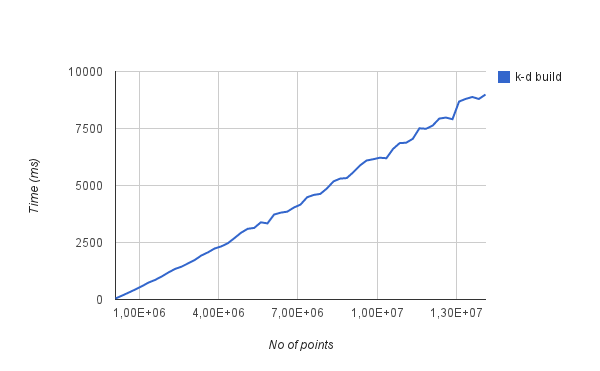
\includegraphics[width=120mm]{../gfx/serial-build.png}
    \caption{Timing results for recursive k-d tree building}
    \label{fig:serial-build}
\end{figure}

We observe that constructing a k-d tree for a large number of points is a costly operation. Given a tree of size $1.41^7$ the algorithm uses nearly $9$ seconds to construct the tree. We also note that the timing results seem to scale linearly in relation to the number of points. This relates nicely to calculated time complexity of the algorithm.

Figure \ref{fig:serial-query} shows the timing results for querying a k-d tree of a given size. The k-d tree is queried for one point with $k=1$. Since we are interested in investigating the average performance, $10^5$ consecutive queries was timed, and the average value for one query was calculated.

\begin{figure}[ht!]
    \centering
    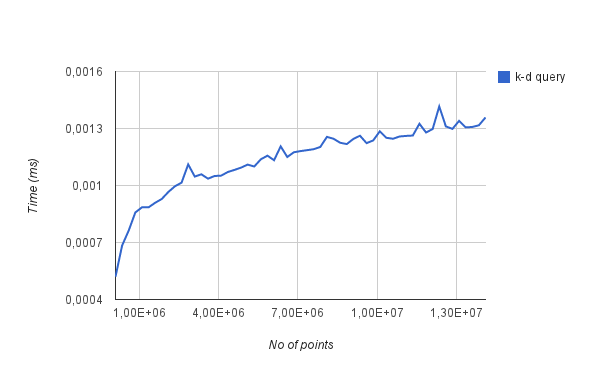
\includegraphics[width=120mm]{../gfx/serial-query.png}
    \caption{Timing results for mean query time with k equal to one}
    \label{fig:serial-query}
\end{figure}

We see that querying the k-d tree is very fast on average. Querying for one point in a tree of size $1.41^7$ takes about $0.0014$ milliseconds. It has to be taken into account, that a query with $k=1$ will give the best query time, since the time complexity of the query algorithm scales with k. Still, for queries with a low $k$, we should expect good performance. The graph also seems to scale with the logarithm of the number of points, as expected by the time complexity calculation.

In order to try to answer RQ~\ref{rq:serial-kd-tree}, we compare the timing results gained from the fastest brute force algorithm developed in Section~\ref{sub:investigation_of_a_brute_force_approach_based_on_garcia}. Figure~\ref{fig:brute-force-vs-serial-build-query} compare the average time required for building a k-d tree of a given size, and performing a single $k=1$ query, to the time required to compute the same result with the fastest brute force algorithm obtained in Section~\ref{sub:investigation_of_a_brute_force_approach_based_on_garcia}.

\begin{figure}[ht!]
\centering
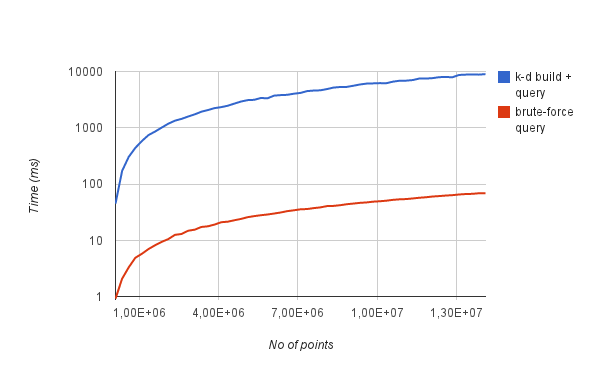
\includegraphics[width=120mm]{../gfx/brute-force-vs-serial-build-query.png}
\caption{Comparison of mean query time with k equal to one with fast brute force and recursive k-d tree based algorithms}
\label{fig:brute-force-vs-serial-build-query}
\end{figure}

In this comparison, the k-d tree based algorithm does not seem like a good option. When performing just one query, the additional time required to build the k-d tree heavily outweighs the benefit of the improved query time, compared to the brute force solution. This result is to be expected, since we are not really utilizing the benefit of the k-d tree, but it is still an important point that a brute force algorithm can be very efficient for certain use-cases.

Let us finally look at some results more closely related to the use-case given by TSI\@. Figure~\ref{fig:brute-force-vs-serial-build-n-queries} does the same comparison as Figure~\ref{fig:brute-force-vs-serial-build-query}, but instead of comparing the time taken to perform one query, $n$ repeated queries are performed, with $n$ being the size of the k-d tree.

\begin{figure}[ht!]
    \centering
    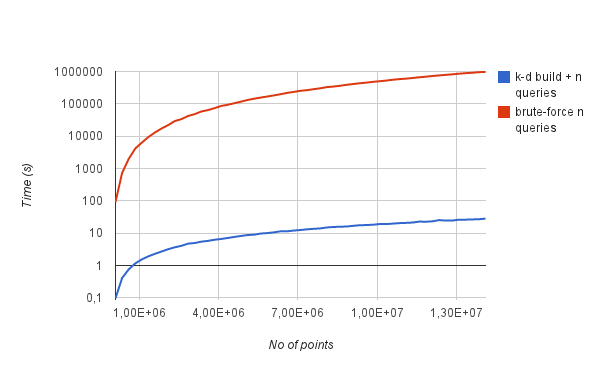
\includegraphics[width=120mm]{../gfx/brute-force-vs-serial-build-n-queries.png}
    \caption{Comparison of timing of n queries with k equal to one with fast brute force and recursive k-d tree based algorithms}
    \label{fig:brute-force-vs-serial-build-n-queries}
\end{figure}

We observe that in this use-case, the k-d tree based approach have much better results than the brute force based approach. Now the k-d tree only have to be built once, but we benefit from the decreased query time in all $n$ queries. Performing $n$ queries on a point cloud of size $1.41^7$ with the brute force based algorithm takes about $9.7*10^5$ seconds, or about 11 days. With the recursive k-d based algorithm, the same operation can be calculated in just over a minute. Considering the needs of TSI, it seem that this approach is worth developing further into an parallel algorithm.

Despite these initial positive results, some problems are apparent from our initial tests.

The k-d tree building algorithm is very slow. Given that we want to perform kNN queries on larger point clouds than $1.41^7$, finding an efficient parallelization of this algorithm would be very beneficial. This is not as trivial as it might seem, as tree-based algorithms do not lend themselves very well to trivial parallelization.

When scaling the number of repeated queries from one to $n$ we observed the huge impact a seemingly small change in the time required for performing one query had on the time needed to compute the entire result. A change from several milliseconds to a fraction of a milliseconds might seem trivial, but given enough repeated queries, this was the difference between minutes and days of computation time. Will we be able to keep the query time down when increasing the value of $k$, and moving the computation over to the GPU, which generally has a slower clock cycle than the CPU.

In the next sections we will address these challenges, along with others, and develop a parallel algorithm for performing kNN queries based on k-d trees.
% subsection testing_a_serial_k_d_tree_based_knn_solver (end)
% % section kd_tree_based_effort (end)

\section{Development of a parallel k-d tree build algorithm} % (fold)
\label{sec:development_of_a_parallel_k_d_tree_build_algorithm}


As noted in the previous section, the k-d tree build process is by far the most expensive operation, and we would save a lot of time by managing to parallelize it. One could think, why not use the serial build algorithm. This is a intuitive choice, but in a CUDA context a recursive algorithm is hard to parallelize. CUDA is based on a massive number of lightweight threads, and to get a fast algorithm one have to split the work between as many threads as possible. This is only possible if it is easy to split and divide the work to independent subtasks. In a recursive context this is hard, because a algorithms execution flow in hidden inside a threads call stack. This makes it hard for other threads to get the information needed to participate. The opposite of a recessive algorithm in an iterative approach, with have a more globally accessible execution flow. This introduces a new resource question.

\begin{myrq}
\label{rq:parallel_build}
    It is possible to parallelize the k-d tree build algorithm, in such a way that it gives a significant speed improvement compared to the serial algorithm.
\end{myrq}

In order to investigate RQ \ref{rq:parallel_build}, we have to look a bit closer at the different steps of the k-d tree build algorithm and look at different parallelization strategies.

Steps:
\begin{enumerate}
    \item Find the median of the points along a specified axis. This median point becomes the value of the current node.
    \item Sort all points with lower values than the median to the left of the median, and all the points with higher values than the median to the right.
    \item Perform this algorithm recursively on the left and right set of nodes.
\end{enumerate}

If we analyze the algorithm \ref{alg:seriel_tree_build}, we can see that for each node in the k-d tree a median finding and a partition has to be made, as described in step 1 and 2. We can call this recursive step a node task. The node task has to be done for all nodes starting at the root and successively go down the tree.



\subsubsection{Parallelization strategy} % (fold)
\label{ssub:parallelization_strategy}


First a good overall parallelization strategy has to be found. A good strategy manage to easily split the main task into small individual subtasks. From the serial recursive algorithm \ref{alg:seriel_tree_build}, we see that there are two recursive calls. This is logical, because we are building a binary tree.  The interesting observation is that a node task is only dependent on the parent node tasks. This means that each tree level are independent, which acts as a good start for our parallelization strategy.

Some other small observation, in regard of a parallelization strategy, is that all subtrees in the k-d tree generation are independent. Hence, the tree corresponding to the left and right child of a node can be done in parallel without any communication. The data is also independent, as a result of how we represent the tree as an array. By data independent, it is meant that the data structure easily can be partitioned to each subtask. In our case will the tree array successively be partitioned into contentious sublists, one for each node task.

From these observations, several strategies can be used to parallelize the k-d tree build algorithm. From the first observation a trivial strategy is to divide the tree levels into dependent tasks, where each node task in a tree level is a independent subtask. This gives us an power of two increasing number of parallel nodes tasks as we increase the tree level. The sublist size will decrease with a factor of two in each downward step. An other strategy is to parallelize each node task.

Both strategies can be used in conjunction with each other. The parallel node task algorithm can be used to speed up the early iterations, where the amount of node task in a tree level is small. As well as further parallelize the subtasks in later tree level iterations. This strategy also fit well to our choice of tree representation. One parallel operation can now take the tree array, split the tree into the current subtrees, perform the node task in each subtree in parallel, and the next tree level is created. All can be done inplace, so the algorithm is as memory efficient as possible.


% subsubsection parallelization_strategy (end)

\subsubsection{From recursive to iterative implementation} % (fold)
\label{ssub:from_recursive_to_iterative_implementation}

\begin{algorithm}
\caption{Iterative k-d tree build}
\label{alg:iterativ_tree_build}
\begin{algorithmic}
    \Function{Build-KD-Tree}{$Tree$}
        \ForAll {$level \in \text{all levels in } Tree$}
            \ForAll{$node \in level$}
                \State $dimension \gets |level| \bmod k$ \Comment{k = 3 for a three dimensional k-d tree}
                \State $\text{Balance-node}(node, dimension)$
            \EndFor
        \EndFor
    \EndFunction
\end{algorithmic}
\end{algorithm}


% subsubsection from_recursive_to_iterative_implementation (end)




% TODO: Header must be improved
\subsubsection{Selecting an algorithm} % (fold)
\label{ssub:selecting_a_algorithm}



As we have seen in section \ref{sub:application_of_kd_trees_to_the_knn_problem}, many algorithms for finding median exist. Since we now want to implement the algorithm with CUDA, the environment has changed, and quick select may not be the best alternative anymore. The first problem with quick select is that it is recursive, which makes it hard to parallelize on CUDA. Therefor it may be profitable to look at other, more parallelization, algorithms.


First a reuse of the bitonic sort was investigated. Given a sorted list one can find the median directly, by simply looking at the midmost element of the array. The partitioning is also done in the process. Unfortunately this strategy proved unsuccessful, as re-purposing the bitonic algorithm for such an task proved difficult. The reason for this is that a pure bitonic sort only manage to sort lists with a length of power of two. The normal solution is to create a longer list then needed, which destroys many of the advantages with our binary tree representation. There are also other solutions to the problem, for example one by K.E. Batcher \cite{Batcher:1968}, but these solutions introduces a lot of divergence that destroys performance on the GPU. We also have the inherent downside of sorting a list in order to find the median, since \BigO{n} algorithms for finding the median exist, compared to the \BigO{n log(n)} time required by sorting.


The existing linear algorithms for finding the median is mostly based on a more generic problem, namely selection or k'th order statistic algorithms \citep[Chapter 9]{Cormen:2001}. Our serial choice, Quick select, is one of these. It is possible to implement a iterative version, so that the bad properties from the recursive version are eliminated. This option was ignored, because literature states that there are other better suited algorithms, like Alabi \citep{Alabi:2012}. Alabi goes through the radix select and bucket select algorithm in detail. The big difference between them is the constant time penalty. The radix sort have a more exact time complexity of \BigO{bn}, where b is the number of bits in each number. While the penalty for bucket select is \BigO{an}, where $a$ stands for the degree of agglomeration in the values. The algorithm is week when the points are clusters together. His results shows that bucket select normally is slightly faster, except when $a$ is high. Although bucket select normally have better results, we expect a high degree of agglomeration in our application, so we choose radix select.


\subsubsection{Radix select} % (fold)
\label{ssub:radix_select}

% subsubsection radix_select (end)

The radix select is based on a bitwise partitioning, much like radix sort \cite[Chapter 8.3]{Cormen:2001}. In each step, elements are partitioned in two subgroups based on the current bit. Then the subgroup that contains the median is determined, and the search continue in that subgroup until the median is found.

\begin{figure}[ht!]
\centering
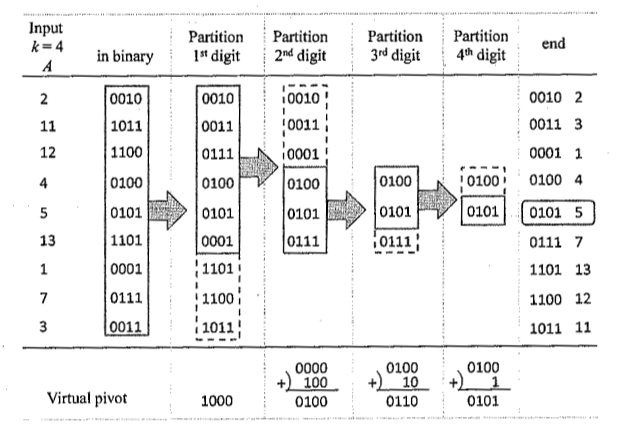
\includegraphics[width=100mm]{../gfx/Radix_select.png}

\caption{An illustration of radix selection \cite{cayman:2012}.}
\label{fig:radix_select}
\end{figure}

When it comes to create a parallelization strategy for radix select it is first advisable to take a look at a highly optimized radix sort like, \citep{MerrillG11}. The radix select can easily be reduced from a radix sort, and many concepts can therefore be reused. An other interesting implementation is the radix select from \citep{Alabi:2012}. They both uses a intuitive parallelization strategy by splitting each radix partition into parallel operations. The way our and Alba's solution differs from Merrill is firstly that we start on the most significant digit, since a least significant digit approach will not reduce the problem in each step. Secondly we only iterate on the digit which contains the median, and let us reduce the problem in each iteration.

Our radix select is a slightly modified version in three ways. We want to solve the node task, which forces us to also partition the list around the median. The algorithm also need to work in a inplace fashion. The last modification, is that our parallel operation must to several radix selections at once, at different parts of the main tree array.


\subsubsection{Our implementation} % (fold)
\label{ssub:our_implementation}


- split up the work in respect to cuda
- Pseudocode
- forklarting av cuda
- diskutere minnebruk. shared memory
- divergence
-



% subsubsection our_implementation (end)





% It is hard to use all the parallel power of cuda in this algorithm. The reason is that the problem is divided in three different types; partition one huge list, partition some middle sized list and partition many small lists. This is the reason why we have chosen to use three different implementation of k'th order statistic. The constant time penalties of the two algorithms we have chosen give us a clear indication the radix select is best on large lists while quick select is best on small lists.

% Results:
% \begin{figure}[ht!]
% \centering
% 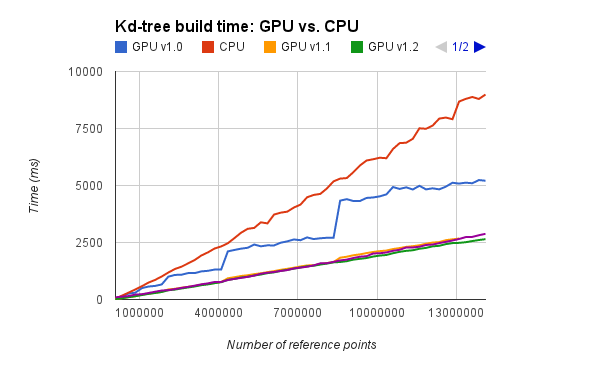
\includegraphics[width=120mm]{../gfx/gpu-vs-cpu-build-time.png}

% \caption{GPU vs CPU build time.}
% \label{fig:sublime_ide}
% \end{figure}

% We see that the parallel implementation performs better than the base serial implementation, building a tree of 14 million points in just over 5 seconds, compared to just under 10 required by the serial algorithm. Still we regard this as a quite rough implementation, in need of more tuning to really bring out the speed potential. The potential for parallelizing the workload for the first and last iterations have not been fully developed. This is due to the implementation forcing one version of the radix select algorithm being to work on all problem sizes. This is not optimal for dividing cuda resources, and as a result, we get high penalties when the problem size reaches unsuitable values.

% We also see a couple of large jumps in the graph. This happens when the number of elements passes a power of two and the height of the resulting k-d tree increase. The height increase hits the implementation at its weakest.

% Tuning the algorithm to alternate between radix select and quick select, eliminates this problem, as is visible in the graph for GPU v1.1. This removes the penalty for calculating the median at unsuitable problem sizes, giving an build time of ~2.4 seconds for 14 million points, compared to the ~9 seconds required by the serial implementation, or the ~5.2 seconds required by the old parallel implementation.

% % subsubsection selecting_a_algorithm (end)
% Memory usage:

% To analyses the space complexity of the k-d tree build and search algorithm, we have made an theoretical calculation of both algorithms GPU memory consumption, and tested it against results from a GeForce 560ti and a Nvidia grid K520 (amazon web service delved).

% It is important to note that the only hard memory limitation is related to building the tree, as a search for N query-points can be performed in several operations. If you e.g. run into memory limitations when searching for pow(10, 8) query-points, you can simply perform two searches on pow(5, 8) query-points to get around the limitation. Loading the pre-built k-d tree on the GPU for searching, and performing one query for a low value of k, will always consume less memory than building the actual k-d tree.

% **Kd-tree-build**

% The memory consumption for the k-d tree build is only depended on the number of points (n) and the theoretical consumption rate grows linearly as \BigO{36n} subset of \BigO{n}.

% \begin{figure}[ht!]
% \centering
% 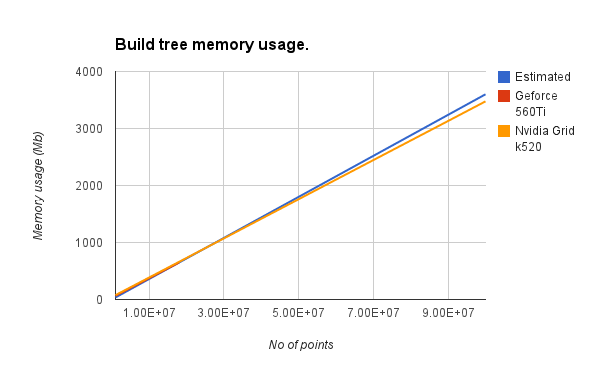
\includegraphics[width=120mm]{../gfx/memory-usage-build.png}

% \caption{Memory usage of k-d tree-build.}
% \label{fig:memory_usage_build}
% \end{figure}

% We see that the estimation fit the real consumption almost perfectly, and with this memory model, we can easily estimate the GPU memory requirements for different problem sizes.

% Given that a customer wants to perform a knn-search on a point cloud of 100 million, he or she would need a GPU with at least 3.6 Gb of spare memory. Under we have tabulated what maximum problem sizes you would expect to be able to run on a selection of Nvidia graphics cards:

% \begin{center}
%     \begin{tabular}{ | l | l | p{5cm} |}
%     \hline
%     Nvidia GPU & Available memory & Maximum problem size \\ \hline
%     GTX TITAN & 6144 MB & 1.79E+08 \\ \hline
%     GTX 780 & 3072 MB & 8.95E+07 \\ \hline
%     GTX 770 & 2048 MB & 5.97E+07 \\ \hline
%     Quadro K6000 & 12288 MB & 3.58E+08 \\ \hline
%     Quadro K5000 & 4096 MB & 1.19E+08 \\ \hline
%     Quadro K4000 & 3072 MB & 8.95E+07 \\ \hline
%     Tesla K40 & 12288 MB & 3.58E+08 \\ \hline
%     Tesla K20 & 5120 MB & 1.49E+08 \\ \hline
%     \end{tabular}
% \end{center}

% These numbers should be read as rough estimates, as each card is expected to have internal processes requiring an unspecified constant amount of the available memory, therefor lovering the maximum problem size possible to run on these cards in practice. It is also worth to mention that when buying a GPU for GPGPU tasks, other performance characteristics is equally, or more, important.

% **Kd-search**

% The kd-search is used to query every point against each other. It has a theoretical memory consumption rate at \BigO({40+4k}n) subset of \BigO{kn}. The consumption is therefore depended on the number of points (n) and the number of neighbors (k).

% \begin{figure}[ht!]
% \centering
% 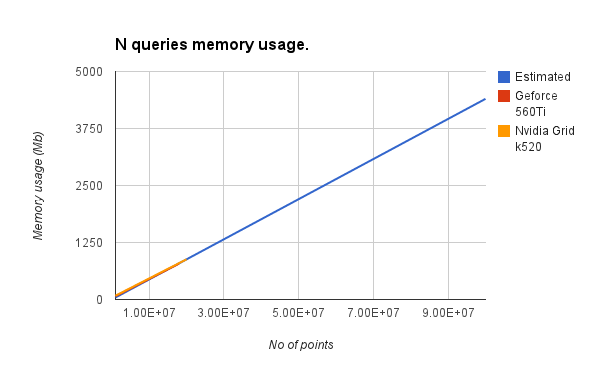
\includegraphics[width=120mm]{../gfx/memory-usage-kd-search.png}

% \caption{Memory usage of kd-search.}
% \label{fig:memory-usage-kd-search}
% \end{figure}

% Also in this case our estimation fit the real consumption with a high degree of accuracy.

% Further work:
% \begin{itemize}
%     \item Look at memory optimization.
%     \item Improve utiliti methods like: accumulateindex, minReduce.
%     \item Forloop Unrolling.
% \end{itemize}

% section development_of_a_parallel_k_d_tree_build_algorithm (end)

\section{Development of a parallel k-d search algorithm} % (fold)
\label{sec:development_of_a_parallel_k_d_search_algorithm}






% Antar begreper qknn har blitt intodusert

Now that a parallel k-d tree build algorithm has been build, lets start looking into a parallelization of the qkNN operation. Some question immediately arise. What is the best way to parallelize such a problem? Will a GPU version give a beneficial speedup? This leads to a new resource question that acts as an expatiation of RQ~\ref{rq:serial-kd-tree}.


\begin{myrq}
\label{rq:parallel_query}
    It is possible to parallelize the qkNN query algorithm, in such a way that it gives a significant speed improvement compared to the serial algorithm.
\end{myrq}


To investigate RQ~\ref{rq:parallel_query}, a real world test and implementation is always beneficial, but first some resource and discussion is needed. Especially in what kind of parallelization strategy and algorithm that should be used. Maybe the GPU is not the right way to parallelize this kind of operations.


\subsection{Parallelization strategy} % (fold)
\label{sub:parallelization_strategy}


The problem at hand is the qkNN search, which is where an assumed big number of query's is to be performed on a k-d tree. At first glance this looks good in terms of parallelization. The main task is naturally divided into individual subtasks, namely the queries. This is a perfect parallelization example, where any number of threads independently can move up and down a constant tree structure.

When CUDA and implementation related questions is introduced, some interesting aspects needs to be addressed. The first is how the work should be divided in terms of CUDA resourced. Should one query be done in a block, should each thread to one query or maybe we should use one thread per $k$ in a query. To address this question, one need to be able to determent if a query itself can be parallelized.

First we see that a query does not have many node visits compared to the size and presumably the number of queries. This ratio is based on the binary logarithm, as for example a tree with one million elements and a $k$ equals one, the number of visited nodes is proportional to $20$. This indicated that many threads is not as beneficial. The relative hard problem of parallelize a query is also a good indicator. Parallelization is, as we have discussed earlier, dependent on individual subtask. The query task is heavily dependent, as the next node is determinant on the previous node. The only place independence comes into existents is where left and right subtree is to be searched, but if this is parallelized the benefit of the pruning is partially destroyed. This leads to one conclusion, if threads is not to be wastefully used, one thread per query is required. In terms of independent tasks, the one thread approach is also logical, since the number of queries should outperform the number of cores on the GPU\@.

The overall parallelization strategy is therefore to use one thread per query and equally distribute the queries amongst the GPU's SM\@.


\subsection{Problem with the recursive implementation} % (fold)
\label{sub:problem_with_the_recursive_implementation}

As discussed in previous sections, GPU's and recursion don't get along well. Previously some drawbacks were mentioned, including the disability for thread communication. Since our parallelization strategy new states that all threads do individually work and don't need to communicate, is there steal a reason for a iterative conversion.

One aspect to consider is connected to how the GPU hardware is constructed. The GPU have a lot of lightweight threads, and has therefor not as mush local space or caching as in a CPU\@. This means that the call stack, where the instructions are manged, is relatively small. A recursive algorithm adds instructions on this call stack at each recursive call. This is the reason why the executions flow of a recursive algorithm is hidden, the call stack is not reachable from the programmers point of view. The big question here is wherever the call stack on a CUDA GPU is big enough for our application.

This question was investigated by a trail and error method, since its hard to do the explicit calculations. The call stack is located locally, so results from a block should be enough. To test the limitations a test that spawned $64$ theoretical threads on an increasing tree size should be sufficient. As the tree size passed \numprint{1e5}, we stared to get unknown errors from CUDA\@. This we concluded was the leak of call stack space and concluded that CUDA had a to small call stack for our purpose.


Divergence is also an accept to consider, and in this case execution divergence. This is, as mention before, then the execution of threads in a warp differs. In a recursive algorithm the decision of whether a recursive call should be made or not, is entirely up to a single thread. Once two threads have made different desiccation, there is no guaranty that they will stay in sync.

The execution divergence can be solved by en iterative solution, where one is guaranteed that every thread always stay in sync. An iterative approach will also solve the call stack problem, where the recursion stack is explicitly stored. The transformation is therefor a necessity.


% subsection problem_with_the_recursive_implementation (end)

\subsection{From recursive to iterative implementation} % (fold)
\label{sub:from_recursive_to_iterative_implementation}


To rewrite Algorithm~\ref{alg:recursive_knn_kd_tree_search} into a iterative algorithm by  explicitly managing the recursion stack, some properties about how the search traverse the k-d tree is needed. From Algorithm~\ref{alg:recursive_knn_kd_tree_search} one can see that this is an inorder traversal, since the current node work is node between the recursive calls. This traversal in also the best strategy in a binary tree search, because the pruning of subtrees is maximized. How to make a standard binary search tree in an iterative fashion is described in Cormen\cite[Chapter 12]{Cormen:2001}, but since this is a k-d tree search the implementation is slightly different, as shown in Algorithm~\ref{alg:iterative_knn_kd_tree_search},

\begin{algorithm}
\caption{Iterative kNN k-d tree search}
\label{alg:iterative_knn_kd_tree_search}
\begin{algorithmic}
    \Procedure{Iterative-kNN-KD-Tree}{$K, r, q$}
        \State \text{Let $S$ be a stack for collecting tree nodes}

        \State $i \gets 2$

        \While{$!S.empty$ \textbf{or} $r$ != NIL}
            \If{$r$ = NIL}
                \State $r \gets \Call{Pop}{S}$
                \State $i \gets r.dimension$

                \If{$r.dx^2 < K.max$} \Comment{Can there be closer points in the other subtree?}
                    \State $r \gets r.other$
                \Else
                    \State $r \gets \text{NIL}$
                \EndIf
            \Else
                \State $d \gets \Call{Distance}{r, q}$

                \If{$d < K.max$} \Comment{Is $r$ closer to $q$ than the current k best points?}
                    \State $r.distance \gets d$
                    \State $\Call{Insert}{K, r}$
                \EndIf

                \State $i \gets (i + 1) \bmod k$ \Comment{k = 3 for a three dimensional k-d tree}

                \State $r.dimention \gets i$
                \State $r.dx \gets r.x(i) - q.x(i)$

                \If{$r.dx > 0$}  \Comment{Select $t$ and $o$ so we traverse towards closest point first}
                    \State $t \gets r.left$, $r.other \gets r.right$
                \Else
                    \State $t \gets r.right$, $r.other \gets r.left$
                \EndIf

                \State $\Call{Push}{S, r}$
                \State $r \gets t$
            \EndIf

        \EndWhile
    \EndProcedure
\end{algorithmic}
\end{algorithm}

The algorithm works in the same way as the recursive algorithm, but adds a stack, $S$, called the s-stack, and a while loop in order to handle the tree traversal iteratively. While there is a element assigned to the root variable, $r$, the algorithm will traverse down the target branch, updating the dimension, $i$, calculating the distance, $dx$, determining the target, $t$, and other, $o$, child node. Then it will collect $r$, $o$, $i$ and $dx$ into one element, and push it on the s-stack. Finally the root variable is assigned to the target child, or NIL if we have reached the end of a branch.

While there still is elements in the s-stack, but $r$ is assigned to NIL, we are traversing back up a branch. While this is happening, the algorithm pops elements from the s-stack, determines if they should be added to the k-heap, before it determines if it need to investigate the other branch of this node. If that is the case, the other node is assigned to $r$, and the algorithm will traverse down this subtree using the previously stated rules.


% subsection from_recursive_to_iterative_implementation (end)

%TODO: Forandre header?
\subsection{The implementation} % (fold)
\label{sub:the_implementation}

To convert our iterative search algorithm to CUDA should now be a trivial matter. The code itself does not need to be parallelized, as only one thread is used per query. The final implementation can be found in Appendix~\ref{sec:cuda_k_d_tree_search} Some key aspects is wort highlighting.


As we converted the algorithm from a recursive to a iterative stack based solution, a lot of the problematic divergence was taken avoided. But as shown in Algorithm~\ref{alg:iterative_knn_kd_tree_search}, there is steal some divergence. This is inevitable since the target subtree and other subtree needs to be treated differently. Although, there are possibilities to minimize the thread branching. If threads in a warp is traversing completely different parts of the tree, they will access different nodes. This is called data divergence. They will also be a minimal change for the threads to synchronize there target and other traversing. The solution is to let each warp search for points that are close in 3-d space, which will force the threads to traverse fore or less together. In our application, query for all points in the k-d tree, this is an easy task. When the k-d tree was build the points are, due to the data structure and the nature of a k-d tree, grouped together relatively to their position in space. The divergence will therefore be minimized if the points are fed to the search as they are placed in the k-d tree.


The transformation from a hidden recursive stack to a explicit stack makes a interesting question about where to store the new stack, especially
since it definitely would have overfilled the local call stack space. This is data that are modifiable and thread independent, which means that the memory options are shared memory, local memory and global memory. Local memory is the memory each thread dynamically can allocate from the heap. First of all, global memory is a working candidate. It has enough space, it is modifiable and accessible to all threads. The huge drawback is the access time, it takes around $400$ clock cycles(Trenger vi cite), and it would be beneficial to use some other kind of memory. Shared memory would be a perfect candidate, because the memory is fast and the need to communicate between blocks is nonexistent. The only drawback needed to address the the amount of data available in shared memory, which is default around $49 kb$ for each block on current NVIDIA GPU's. This is also a good approximation for how much local memory available.

The two stacks in question is the k-stack and the transformed recursive stack, called stack from now on. Both stacks are memory wise dependent on number of threads, since each thread needs unique stacks. The stack is dependent on how many elements the inorder tree traversal needs to store. If one looks on how the algorithm handles the stack, one can see that elements are pushed on the way down, and poped when one traverse upwards.  This means that the stack never will be longer then the tree hight, which is the binary logarithm if the size. One stack element uses $16$ bytes of space, which means that the stack memory is s subset of $\Theta(16\log_2(n)T)$. Here $T$ represent the number of threads and $n$ is the k-d tree size. The k-stack depends on the number of closest neighbors, $k$, and one element uses $8$ bytes. This implies that it uses memory usage will look like, $\Theta(8kT)$.


\begin{figure}[ht!]
\centering
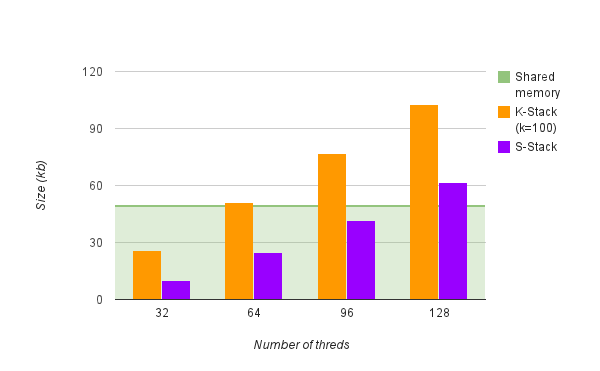
\includegraphics[width=100mm]{../gfx/shared_memory_and_stack.png}

\caption{The stacks memory usage compared to the amount of shared memory.}
\label{fig:stacks_and_shared_memory}
\end{figure}


In Figure~\ref{fig:stacks_and_shared_memory} the memory usage of each stack is compared to the available shared memory. Some basic assumptions and approximations have been done in regard to the data. Treads are only compared in multiples of $32$, since this is the warp size and is therefore the most optimal thread numbers. The value of $k$ is dependent on the problem in hand, and as our application only needs a value of $100$, that value is used. When it comes to the logarithm in the stack calculations, we have chosen $30$.  This is because it value is relatively constant and with a value of this type we support a \numprint{1e9} big k-d tree.


Figure~\ref{fig:stacks_and_shared_memory} shows that the k-stack is not a suitable candidate. Already at a thread count of $64$ the memory is used. The highly dependent and variably $k$ value also make the stack size unpredictable. The stack however looks really promising, with $64$ threads the memory usage is well below the limit. This also shows that local memory a suitable candidate, since it allocate memory from the same L1 chip as the shared memory.

\begin{figure}[ht!]
    \centering
    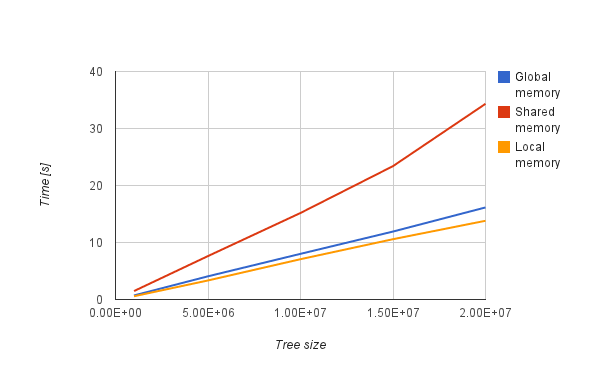
\includegraphics[width=100mm]{../gfx/stack_speed.png}

    \caption{Speed comparison between different stack memory types. The test are done with $k$ equals 10 and \numprint{1e6} queries per tree size. }
    \label{tbl:stack_speed}
\end{figure}



To decide what kind of memory is optimal for our stack, Figure~\ref{tbl:stack_speed} has been created. Surprisingly shared memory looks like the slowest alternative, even though the two other should be stored in global memory. Shared memory is synced between all threads in a block, and may have some of the blame for our results. One property of the stack is that it is completely thread local, meaning communication between threads is not needed. The extra, and wasted property of the shared memory may lead to to a decrease in latency, because data is synced between the threads.

An other reason is that there is some kind of programming error, and some part of a stack was used by two threads. This would lead to a lot of write and read collisions, and cause a lot of time penalties. The programming error would also lead to wrongly results, which is not the case and the error possibility is ignored.

Although global and local memory presumably is stored at the same place, the are some noticeable differences that can explain the time gap between them. The cache may be a noticeable factor. The cache is is placed on the same on-chip memory as the shared memory, and should therefore be equally fast. The difference is that cashing is not programmable and therefor not controlled be the programmer. However some properties in the local memory type may suggest that it is a more likely candidate to be cached.  The local memory is thread dependent and is not accessible to other threads or blocks as the global memory are. The compiler can therefor logically imply that the data is not modified by other threads and caching becomes mush more likely. Figure~\ref{fig:stacks_and_shared_memory}, also shows us that the cache can fit all stacks in a block, which correlates with the timing results. To enforce cache use even further CUDA gives a runtime function call to give more of the on-chip memory to caching.

The discussion and results for the stack analysis shows that the stacks highly impact the timing results. This means that the k-stack is also a dominant  speed factor, as corresponds well to the k-stack tests that was performed. Two k-stack variants was tested. One that used a bobble sort\cite{Cormen:2001} like implementation. It works by always keeping a sorted list. An element is inserted by, from the bottom position, swapping it to the adjustment element until it is in the right place. The other method is based on a heap sort implementation, that is explained in Section~\ref{sub:querying_the_k_d_tree}. The timing difference between the two implementations was around $5$ times. The fastest one was of course the heap-sort variant, since it need to access mush less elements. The difference is the insertion time complexity, where the bobble variant is a \BigO{n} and the heap sort variant is a \BigO{log_2(n)}.


\subsubsection{Open-MP} % (fold)
\label{ssub:open_mp_version}

The high impact the stack had on performance make an interesting question in regard to RQ~\ref{rq:parallel_query}. Could a parallel implementation in the CPU outperform the CPU version? When the latency effect, as the stacks showed, had such a huge impact on the performance. The CPU has a lot more cache then the GPU and would therefor not be affected that mush. The real question is whether the CUDA implementation manges to hide the latency problem by alternating between different warps.

For this to be investigated properly, an OpenMP version of the k-d tree search has to be created. Parallelization wise this is not as different as in our CUDA discussion, and there are only some implementation details to address. The big discussions around what kind of memory to use or memory size can also be ignored, since the CPU has enough cache and the latency is not that important. The implementation can be found in Appendix~\ref{sec:open_mp_k_d_tree_search}.

% subsubsection open_mp_version (end)


% subsection our_implementation (end)











% \begin{figure}[ht!]
% \centering
% 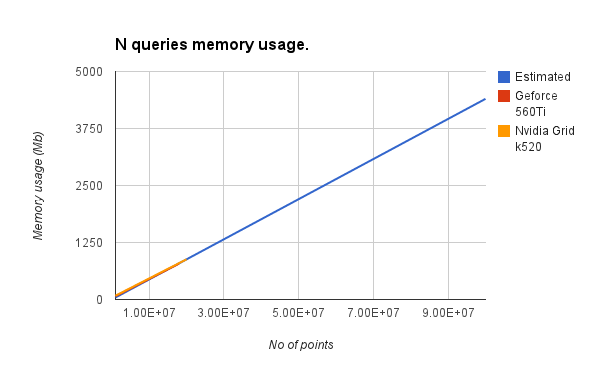
\includegraphics[width=120mm]{../gfx/memory-usage-kd-search.png}

% \caption{Memory usage of kd-search.}
% \label{fig:memory-usage-kd-search}
% \end{figure}

% Also in this case our estimation fit the real consumption with a high degree of accur
% Further work:
% \begin{itemize}
%     \item Look at memory optimization.
%     \item Improve utiliti methods like: accumulateindex, minReduce.
%     \item Forloop Unrolling.
% \end{itemize}





% section development_of_a_parallel_k_d_search_algorithm (end)

\section{CUDA Optimizations} % (fold)
\label{sec:cuda_optimizations}

Throughout this quest many optimizations have been done, some focusing on the algorithmic aspect, others more on implementation. This section is focusing on different CUDA optimizations and why it is necessary in regard of performance. Some performance considerations, like divergence, have already been mentioned, due to it's direct relation to the different implementations. Other important factors, occupancy, coalescing, loop-unrolling, block and thread load balancing.
% TODO: Add arithmetic operations in list?

Occupancy is a metric, which relates to how many active warps there are on a SM. Earlier we have talked about how thread instructions are executed sequentially, resulting in alternating warps, one warp is paused while the other is executing. The time a stalled warp will use to retrieve data, increases with the number of warps per SM. One should note that high occupancy does not always result in high performance, but low occupancy will always result in an inability to hide latency, which result in bad performance.

The struggle to always have the right amount of occupancy, also relates to dividing CUDA resources. As well as keeping a right amount of warps in a SM, one must also keep every SM in activity. Forcing the algorithm to work over unsynchronizable blocks. The number of blocks, that are optimal to keep in activity, changes with different GPUs. It is therefore important to think of how many blocks and threads that are launched with each kernel. We have solved this issue with methods that, based on different algorithmic parameters, calculates how many threads and blocks are needed for a particular launch.

To coalesce memory access to global memory, is probably one of the most performance increasing optimizations in CUDA, especially in our memory intense application. Global memory that is loaded and stored by threads in a warp, can be coalesced into only one transaction, if the right conditions are met. How a device coalesce memory depends on the compute capability, but some basic properties are common. A warps access will coalesce into onto a number of transactions that equals the number of cache lines needed to service all the threads in the warp. Devices with compute capability $2.x$ will by default cache directly to L1, which has 128-byte lines. Higher capabilities will always cache to L2 cache, that have 32-byte segments\cite{cuda_c_best_practices_guide}. 

\begin{figure}[ht!]
    \centering
    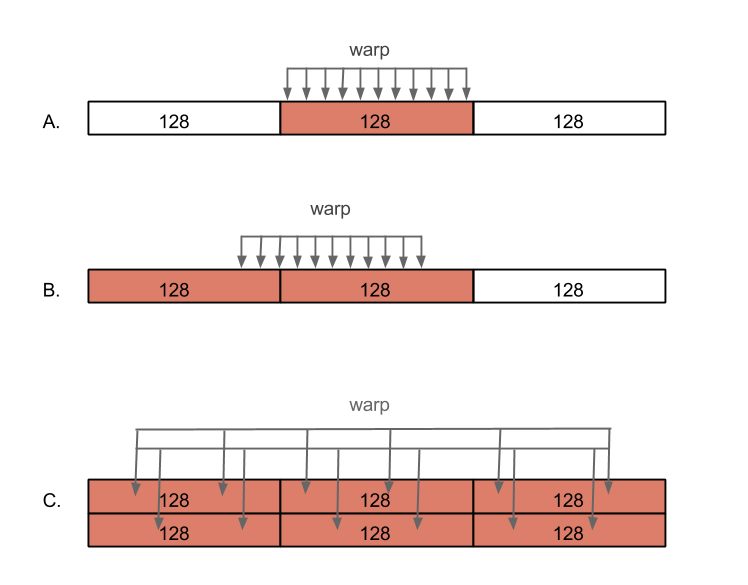
\includegraphics[width=100mm]{../gfx/memory_coalecing.png}
    \caption{Three different memory transactions, where A and B result in good coalesced and cached transactions, while C shows a stride access pattern with bad coalescing.}
    \label{fig:coalesing_memory}
\end{figure}

If we focus on compute capability 2.x, Figures~\ref{fig:coalesing_memory}, shows have memory are coalesced. Green indicate memory lines that are retrieved, while blue indicate non retrieved lines. The first figure illustrate perfect coalescing, a warp performs a sequential 128-byte transaction that fit perfectly in a 128-byte lines. The second shows a misaligned sequential retrial, resulting in two transactions. The third uses stride access pattern with a offset of $128$ resulting in bad coalescing.

We have tried to maximize coalescing by always using sequential addressing. This kind of addressing can be achieved in many ways. One way, that we have use throughout the code, is based on how data are partitioned and iterated. The generic partitioning algorithm, Algorithm~\ref{alg:general_aspects_dividing}, that we used to expand Garcia's algorithm, shows how this could be done.     


The last optimization keyword we would like to introduce is unrolling. This is a technique we have used on many of our algorithms, like min-reduce, and also in some of our utility functions, like for example to accumulate an array. Unrolling is a standard technique in ordinary high performance serial programming, optimizing pipelining, and is given an extra dimensions on CUDA\@. 

Loop unrolling, is the procedure of rewriting a loop, containing conditional operators, into hard-coded sequential steps. This way, the result of conditional operators may be determined at compile-time, eliminating branching of the control flow. On a CUDA context this is of course the case, but in addition it will minimize divergence.

The idea of loop unrolling can also be applied to warps. This is called warp unrolling, and it can be used if we know we are in a single warp. The results being, that no expensive thread synchronization is needed, since every warp is accessing a unique memory location.

%TODO: Skal denne være med?.
A last note to add is arithmetic operations. Some arithmetic operations are more costly then others, like modulo and divisions. It is therefore time saving to optimize, in computationally heavy algorithms. This is especially the case in the light weighted threads found in CUDA. For instants, one can use a right bit-shift to divide a number by two.

% section cuda_optimizations (end)

\cleardoublepage
